\section{Optimum Filters}
A optimum filter minimize the mean-square error $\xi = E\left(|e(n)|^2\right) \quad x(n)=d(n)+v(n) \quad e(n) = d(n) - \tilde{d}(n)$\\
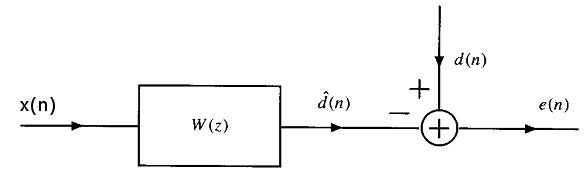
\includegraphics[width=9cm]{../StatDig/bilder/optimumFilter.jpg}\\
The minimal error is \textbf{always orthogonal} to the data: $E(e(n)x^*(n-k))=0$ $\forall$ $k\epsilon[0,p-1]$

\subsection{Wiener FIR Filter \hayes{337}}
\begin{minipage}{10cm}
\begin{tabbing}

Wiener-Hopf equations: \= $\sum \limits_{l=0}^{p-1} w(l)r_x(k-l)=r_{dx}(k)$; $\forall$ $k\epsilon[0,p-1]$ \\
Correlations:  \>
						$r_x(k)=E \{ x(n)x^{*}(n-k) \}$ \\
\>						$r_{dx}(k)=E\{d(n)x^{*}(n-k)\}$ \\
Minimum Error: \>		$\xi_{min}=r_d(0)-\sum \limits_{l=0}^l w(l)r_{dx}^{*}(l)$
\end{tabbing}
\end{minipage}
\begin{minipage}{10cm}
$\small
\underbrace{\begin{bmatrix}                   
    		r_x[0] & r_x^*[1] & \hdots & r_x^*[p-1] \\   
    		r_x[1] & r_x[0] & \hdots & r_x^*[p-2] \\    
    		\vdots & \vdots & \ddots & \vdots \\     
    		r_x[p-1] & r_x[p-2] & \hdots & r_x[0] \\ 
		\end{bmatrix}  }_{R_x} \cdot \underbrace{\begin{bmatrix}
    		w(0) \\
    		w(1) \\
    		\vdots \\
    		w(p-1)
		\end{bmatrix}  }_{w}= \underbrace{\begin{bmatrix}
    		 r_{dx}[0]\\            
    		 r_{dx}[1]\\
    		\vdots \\
    		 r_{dx}[p-1]\\
		\end{bmatrix}}_{r_{dx}} 
		 $$ \normalsize	 $\\
$$R_x \cdot w =r_{dx}$$
\end{minipage}
\begin{minipage}{7.5cm}
\subsubsection{Filtering \hayes{339}}
The input signal is $x(n)=d(n)+v(n)$. Because the noise and the data signal is uncorrollated and the noise has zero mean, the Wiener-Hopf equation simplify follow:\\
$r_x(k)=r_d(k)+r_v(k) \rightarrow [R_d + R_v]\cdot w = r_d$\\
 with $R_v=\small \begin{bmatrix}                   
    		\sigma_v^2 & \hdots & 0\\   
    		\vdots & \ddots & \vdots \\     
    		0&  \hdots &\sigma_v^2 \\ 
		\end{bmatrix} $
\end{minipage}
\hspace{5mm}
\begin{minipage}{10cm}
\subsubsection{Linear Prediction FIR \hayes{342}}
$\hat{x}(n+\alpha)=\sum \limits_{k=0}^{p-1} w(k)[x(n-k)+v(n-k)]$

$ 	\hookrightarrow  	\small \begin{bmatrix}                   
    		r_y[0] & r_y^*[1] & \hdots & r_y^*[p-1] \\   
    		r_y[1] & r_y[0] & \hdots & r_y^*[p-2] \\    
    		\vdots & \vdots & \ddots & \vdots \\     
    		r_y[p-1] & r_y[p-2] & \hdots & r_y[0] \\  
		\end{bmatrix}   \cdot \begin{bmatrix}
    		w(0) \\
    		w(1) \\
    		\vdots \\
    		w(p)
		\end{bmatrix} = \begin{bmatrix}
    		 r_{x}[\alpha]\\            
    		 r_{x}[\alpha+1]\\
    		\vdots \\
    		 r_{x}[\alpha+q]\\
		\end{bmatrix}
$$ \normalsize	 $\\
$\alpha$ are the steps to predict. Noise: $r_y(k) = r_x(k) + r_(k)v$\\
\end{minipage}\\
\begin{minipage}{11.5cm}
\subsubsection{Linear Phase Filter \hayes{17}, exercise 9.16} 
All frequency are delayed same. \\
For \textbf{FIR}: the coefficients are symmetric $(z^1+2z^0+z^{-1})$ or with a causal filter: $z^0 + 2z^{-1} + z^{-2}$\\
$\small \begin{bmatrix}
2 r_x[0] + 2 r_x[2]		&	2 r_x[1] \\
2 r_x[1]				& 	r_x[0]
\end{bmatrix} \cdot \begin{bmatrix}
w_n(1)\\
w_n(0)
\end{bmatrix}= \underbrace{ \begin{bmatrix}
r_x[\alpha] + r_x[\alpha+2]\\
r_x[\alpha+1]
\end{bmatrix}}_{\text{for linear prediction} } 
= \underbrace{ \begin{bmatrix} = 
r_{dx}[0] + r_{dx}[2]\\
r_{dx}[1]
\end{bmatrix}    }_{\text{for optimal filter} }  $

\end{minipage}
\hspace{3mm}
\begin{minipage}{7cm}
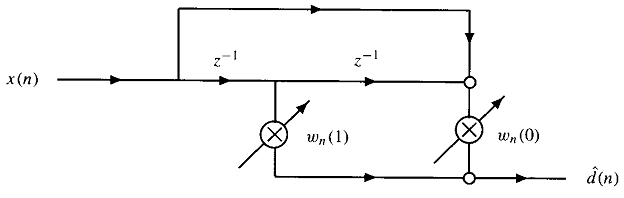
\includegraphics[width=7cm]{../StatDig/bilder/linear_phase_fir.png}
How a linear phase FIR filter 2 order is implemented in hardware.
\end{minipage}
\subsection{Wiener IIR Filter}
\begin{minipage}{8cm}
\subsubsection{Noncausal \hayes{353}}
\begin{tabbing}
Wiener-Hopf equations: \=
$H(e^{jw})=\frac{P_{dx}(e^{jw})}{P_{x}(e^{jw})}  \Rightarrow
\frac{P_{d}(e^{jw})}{P_{d}(e^{jw}) + P_{v}(e^{jw})}= \frac{SNR(e^{j\omega})}{SNR(e^{j\omega}) + 1}$ (often called \textbf{the} Wiener Filter) \\

Correlations: \>
	$r_x(k) =E \{ x(n)x^{*}(n-k) \} $\\ 
	\>$r_{dx}(k) =E\{d(n)x^{*}(n-k)\}$\\


Minimum Error:\>
	$\xi_{min} =r_d(0)-\sum \limits_{l=-\infty}^\infty h(l)r_{dx}^{*}(l)$
	=$\frac{1}{2\pi}\int \limits_{-\pi}^\pi[P_d(e^{jw})-H(e^{jw})P_{dx}^{*}(e^{jw})]dw$
\end{tabbing}

\end{minipage}

\subsubsection{Causal \hayes{358}}
\begin{tabbing}
Spectral Factorization: \=
$ P_x(z) = \sigma_0^2 Q(z) Q^*(z^{-1}) $\\

System function:\hspace{1.2cm}\>
	$H(z)=\frac{1}{\sigma_0^2 Q(z) } [\frac{P_{dx}(z)}{Q^*(z^{-1})} ]_+ $ \\
	
Minimum Error:\>$\xi_{min} =r_d(0)-\sum \limits_{l=0}^\infty h(l)r_{dx}^{*}(l)
	=\frac{1}{2\pi}\int \limits_{-\pi}^\pi[P_d(e^{jw})-H(e^{jw})P_{dx}^{*}(e^{jw})]dw$\\
	
\end{tabbing}
Example \hayes{362}

\subsubsection{Linear Prediction IIR \hayes{365}}
\begin{tabbing}
System function:\hspace{0.2cm}\=
	$ r_{dx}(k)=r_x(k+\alpha)  \qquad \alpha \text{ = steps to predict.} $\\
\>	$ H(z)= \frac{1}{Q(z)}[z^\alpha Q(z)]_+ $ \hspace{6.8cm} \=$\rightarrow \text{monic, one step } H(z) = z [1- \frac{1}{Q(z)}] $\\
Minimum Error:\>
	$\xi_{min} =r_d(0)-\sum \limits_{l=0}^\infty h(l)r_{dx}^{*}(l)
		=\frac{1}{2\pi}\int \limits_{-\pi}^\pi[P_d(e^{jw})-H(e^{jw})P_{dx}^{*}(e^{jw})]dw $\>$ \rightarrow \text{monic, one step } \xi_{min} = \sigma^2_0$\\
\end{tabbing}


\subsubsection{Wiener Deconvolution \hayes{369}}
Deconvolutate a signal $x(n)=d(n)\ast g(n) + w(n)$ (not $x(n)=d(n) + g(n)$) it's not easy. At the best, the signal could be reconstruct as:
$\hat{D}(e^{\omega})=D(e^{j\omega}) + \frac{W(e^{j\omega})}{G(e^{j\omega})}=D(e^{j\omega})+V(e^{j\omega})$ \quad $V(e^{j\omega})$ isn't anymore white noise. 
Espacialy if $G(e^{j\omega})$ becomes small the noise will be amplified.\\
System function:\hspace{1.2cm}
	$ H(z)= \frac{1}{G(z)}\left[\frac{P_d(z)}{P_d(z)+P_w(z)/|G(z)|^2}\right]$\\

\subsection{Discrete Kalman Filter \hayes{371}}
The Kalman Filter is a Best Linear Unbiased Estimator (BLUE).

\textbf{Grundgedanke} Beim Kalman Filter wird der Kalman Gain nach dem
kleinsten Fehlerquadrat geschätzt. Speziell am Kalman ist, dass Messgrössen
mithilfe der Zustandsgrössen und einem Rauschsignal definiert ist. \\
\subsubsection{Voraussetzung}
\begin{aufzaehlung}
   	\item Physikalisches Modell/Systementwicklung (für normales sogar ein
   	lineares Modell)
   	\item Messwerte, auch eine Sensorfusion möglich (mehrere Messwerte für ein
   	Systemzustand)
   	\item für normales Kalman: linearer Zusammenhang zwischen Messwerten und
   	Zustandsgrössen
\end{aufzaehlung}
\begin{minipage}{8cm}
	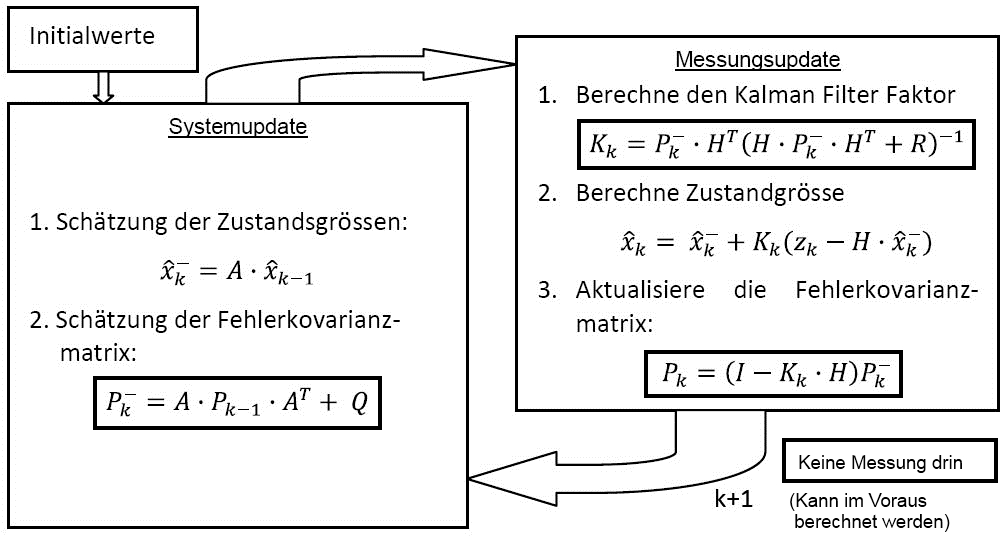
\includegraphics[width=8cm]{Content/AdaptSigVer/KalmanFilter.jpg}
	
	\begin{itemize}
		\item $\hat{x}_{k-1}$ und $P_{k-1}$ benötigen Initialisierungswerte
		\item $P_K$ und $K_K$ können offline vorausberechnet werden, wenn das System nicht ändert
	\end{itemize}
	
\end{minipage}
\begin{minipage}{11cm}
	\small
	\subsubsection{Funktion}
		\begin{liste}
	    	\item A Systementwicklungsmatrize: Physikalische Modell
	    	\item K Kalman Gain: Gewichtet interne Schätzung und die Messungen der
	    	einzelnen Sensoren (0=Nur interne Schätzung;1=nur Messung)
	    	\item H Messmatrize: Zusammenhang zwischen Mess- und Zustandsgrössen
	    	\item P (Fehlerkovarianzma.) Schätzgrösse für den Fehler. Je grösser desto
	    	mehr wird aktuelle Messung berücksichtigt. Beim normalen Kalman Filter
	    	konvergiert dieser mit der Zeit.
	    	\item z: Messwerte (auch von mehreren gleichartigen Sensoren möglich)
	    	\item x: Zustandsgrössen
	    	\item Initialwert: Systemwerte beliebig; Fehlerkovarianzmatrize sehr
	    	gross wählen, so dass zuerst nur die Messung berücksichtigt wird
	    	\item Q Standartabweichung System (Systemrauschen)
	    	\item R Standartabweichung der Sensoren (Messrauschen)
				\item Das Verhältniss von Q zu R ist für die Filtereinstellung verantwortlich.\newline
				$\frac QR$ gross $\rightarrow$ vertraut mehr den Messdaten\newline \hspace{4cm} $\frac QR$ klein $\rightarrow$ vertraut mehr den Systemeigenschaften
	    \end{liste}
	\normalsize
\end{minipage}\\
\clearpage

\subsubsection{Kalman Algorithm}
Idea: Best estimation when process and observer equation as well as some initial conditions are given.
$\mathbf{\hat x}(n|n)$ is the prediction, $\mathbf{P}$ is the error covariance matrix, $\mathbf{K}$ is the Kalman gain.
The index $\mathbf{\hat x}(a|b)$ $a$ stands for the iteration number ($n$ = now) and $b$ is which input
data has to be taken ($n-1$ = data up to the last iteration). 
\begin{alignat}{2}
	&\text{State equation:}\qquad&&\mathbf{x}(n) =\mathbf{A}(n-1)\mathbf{x}(n-1) + \mathbf{w}(n) \qquad 
	 \mathbf{Q}_w = \text{noise covariance matrix} \underbrace{= \sigma_w^2}_{\text{when one dimensional}}  \nonumber\\
	&\text{Observer equation:}\qquad&&\mathbf{y}(n) =\mathbf{C}(n)\mathbf{x}(n) + \mathbf{v}(n) \qquad \qquad \quad \quad
   \mathbf{Q}_V = \text{noise covariance matrix} \underbrace{= \sigma_v^2}_{\text{when one dimensional}} \nonumber\\
	\nonumber\\
	&\text{Initial condition:}	\qquad	&&\mathbf{x}(0|0)=E\{\mathbf{x}(0)\} \qquad \qquad \text{might be zero}\nonumber\\
										&&&\mathbf{P}(0|0)=E\{\mathbf{x}(0)\mathbf{x}^{\mathrm T}(0)\} \qquad \text{should be high}\nonumber\\
	\nonumber\\
	\label{kal1}
	&\text{Prediction:}			\qquad	&&\mathbf{\hat{x}}(n|n-1)=\mathbf{A}(n-1)\mathbf{\hat{x}}(n-1|n-1)\\
										&&&\mathbf{P}(n|n-1)=\mathbf{A}(n-1)\mathbf{P}(n-1|n-1)\mathbf{A}^{\mathrm T}(n-1) + \mathbf{Q}_w(n)\\
	\nonumber\\
	&\text{Update:}				\qquad	&&\mathbf{K}(n)=\mathbf{P}(n|n-1)\mathbf{C}^{\mathrm T}(n)\left[\mathbf{C}(n) \mathbf{P}(n|n-1)\mathbf{C}^{\mathrm T}(n)+\mathbf{Q}_v(n)\right]^{\textbf{\textcolor{red}{-1}}}\\
										&&&\mathbf{\hat{x}}(n|n)=\mathbf{\hat{x}}(n|n-1)+\mathbf{K}(n)\left[\mathbf{y}(n)-\mathbf{C}(n)\mathbf{\hat{x}}(n|n-1)\right]\\
										&&&\mathbf{P}(n|n)=\left[\mathbf{I}-\mathbf{K}(n)\mathbf{C}(n)\right]\mathbf{P}(n|n-1)\\
										&&&\textbf{continue with \eqref{kal1}}	
\end{alignat}

The steady-state is reached when $\mathbf{P}(n|n) = \mathbf{P}(n-1 | n-1)$ and $\mathbf{K}(n) = \mathbf{P}(n|n)$.

\subsubsection{Vereinfachtes Prinzip des Kalman-Filters}
\begin{minipage}{14.5cm}
Man hat zwei ungenaue Sensoren $T_1$ und $T_2$ (unkorreliert), welche das gleiche Signal messen und deren Standardabweichungen $\sigma_1$ und $\sigma_2$ bekannt sind. Der beste
Schätzer $\hat{T}$ wird wie folgt errechnet:\\
\end{minipage}
\hspace{0.25cm}
\begin{minipage}{5cm}
$\hat{T}=\frac{\sigma_1^2}{\sigma_1^2+\sigma_2^2}\cdot T_2+\frac{\sigma_2^2}{\sigma_1^2+\sigma_2^2}\cdot T_1$
\end{minipage}
\begin{minipage}{14.5cm}
Man hat zwei korrelierte Signale $T_1$ und $T_2$ mit $\sigma_1$ und $\sigma_2$ und dem Korrelationskoeffizient $\rho$ bekannt. Der beste
Schätzer $\hat{T}$ wird wie folgt errechnet:\\
\end{minipage}
\hspace{0.25cm}
\begin{minipage}{5cm}
$\hat{T}=k_1\cdot T_1 + k_2\cdot T_2$\\
$k_1=\frac{\sigma_2^2-\rho \sigma_1 \sigma_2}{\sigma_1^2 - 2 \rho \sigma_1 \sigma_2 + \sigma_2^2}$\\
$k_2=1-k_1=\frac{\sigma_1^2-\rho \sigma_1 \sigma_2}{\sigma_1^2 - 2 \rho \sigma_1 \sigma_2 + \sigma_2^2}$\\
\end{minipage}
